%%
%% This is file `docultexmm.tex',
%% Documentation for siam multimedia macros for use with LaTeX 2e
%%
%% December 19, 2013
%%
%% Version 1.0.1
%%
%% You are not allowed to change this file.
%%
%% You are allowed to distribute this file under the condition that
%% it is distributed together with all of the files in the siam macro
%% distribution. These are:
%%
%%  siamltexmm.cls (this file)
%%  siam11.clo   (required size option for 11pt papers)
%%  subeqn.clo   (allows equation numbers with lettered subelements)
%%  siam.bst     (bibliographic style file for BibTeX)
%%  docultexmm.tex (documentation file)
%%
%% If you receive only some of these files from someone, please contact:
%% multimedia@siam.org
%%
%% You are not allowed to distribute this file alone. You are not
%% allowed to take money for the distribution or use of either this
%% file or a changed version, except for a nominal charge for copying
%% etc.
%%
%% \CharacterTable
%%  {Upper-case    \A\B\C\D\E\F\G\H\I\J\K\L\M\N\O\P\Q\R\S\T\U\V\W\X\Y\Z
%%   Lower-case    \a\b\c\d\e\f\g\h\i\j\k\l\m\n\o\p\q\r\s\t\u\v\w\x\y\z
%%   Digits        \0\1\2\3\4\5\6\7\8\9
%%   Exclamation   \!     Double quote  \"     Hash (number) \#
%%   Dollar        \$     Percent       \%     Ampersand     \&
%%   Acute accent  \'     Left paren    \(     Right paren   \)
%%   Asterisk      \*     Plus          \+     Comma         \,
%%   Minus         \-     Point         \.     Solidus       \/
%%   Colon         \:     Semicolon     \;     Less than     \<
%%   Equals        \=     Greater than  \>     Question mark \?
%%   Commercial at \@     Left bracket  \[     Backslash     \\
%%   Right bracket \]     Circumflex    \^     Underscore    \_
%%   Grave accent  \`     Left brace    \{     Vertical bar  \|
%%   Right brace   \}     Tilde         \~}

\documentclass[final,leqno,onefignum,onetabnum]{siamltexmm}

\usepackage{amsmath}
\usepackage{amsfonts}

\usepackage{epsfig}

\title{Data-driven Reduction of Multiscale Stochastic Dynamical Systems \thanks{This work was
supported by ....}}

\author{Carmeline J. Dsilva\footnotemark[2] \and Ronen Talmon\footnotemark[3] \and C. William Gear\footnotemark[2] \and Ronald R. Coifman\footnotemark[4] \and Ioannis G. Kevrekidis\footnotemark[2]\ \footnotemark[5]}

\begin{document}
\maketitle
\newcommand{\slugmaster}{%
\slugger{siads}{xxxx}{xx}{x}{x--x}}%slugger should be set to juq, siads, sifin, or siims

\renewcommand{\thefootnote}{\fnsymbol{footnote}}

\footnotetext[2]{Department of Chemical and Biological Engineering, Princeton University, Princeton, New Jersey, 08544, USA}
\footnotetext[3]{Department of Electrical Engineering, Technion, Haifa, Israel, 3200003}
\footnotetext[4]{Department of Mathematics, Yale University, New Haven, Connecticut, 06520, USA}
\footnotetext[5]{Program in Applied and Computational Mathematics, Princeton University, Princeton, New Jersey, 08544, USA}

\renewcommand{\thefootnote}{\arabic{footnote}}

\begin{abstract}

\end{abstract}

\begin{keywords}\end{keywords}

\begin{AMS}
37M10, 62-07
\end{AMS}

\pagestyle{myheadings}
\thispagestyle{plain}
\markboth{C.~J. DSILVA {\it ET AL}}{DATA-DRIVEN REDUCTION OF SDES}


\section{Introduction}

\begin{itemize}

\item
Bridge/connect between data mining/analysis and dynamical systems

\begin{itemize}

\item
Main idea and scope: analyze stochastic dynamical systems using data-driven methods.

\begin{itemize}

\item
Reduction in fast-slow systems using manifold learning

\end{itemize}

\end{itemize}
\item
We cannot use off-the-shelf data-driven methods because they are typically based on metrics and geometry and are not informed (take into account) the dynamics and time.

\item
Our contribution:

\begin{itemize}

\item
We show how to use data analysis methods that are typically applied to data sets for analyzing data collected as a time series from a dynamical system. In particular, we ``propose" a data-driven (graph-based) method for recovering the slow variable of reducible systems.

\item
The method is based mostly on local analysis that combines geometry and dynamics.

\item
We offer rigorous analysis for the method that gives the conditions (for our method to successfully recover the ``right" slow variables), intuition.

\end{itemize}

\end{itemize}

\begin{figure}[t]

\centering

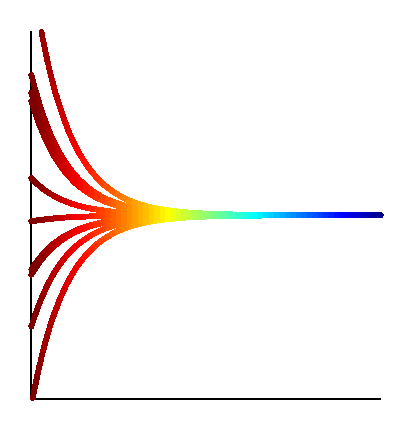
\epsfig{width=2in, file=schematic_DS1.eps}
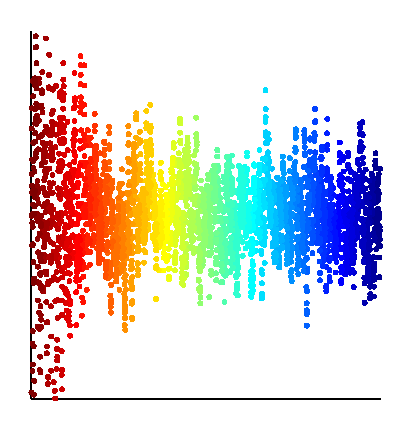
\epsfig{width=2in, file=schematic_DS2.eps}

\vspace{0.25in}

\caption{(Left) Schematic of multiscale system where the value of one variable becomes slaved to the other variable. (Right) Schematic of multiscale system where the statistics of one variable become slaved to the other variable.}
\end{figure}

\subsection{Multiscale Stochastic Systems} \label{subsec:multiscale_SDE}

We assume we have the following two-scale stochastic differential equation (SDE),
\begin{equation} \label{eq:general_SDE}
\begin{aligned}
dx_i(t) &= a_i(\vec{x}(t)) dt + dW_i(t), & \: 1 \le i \le m \\
dx_i(t) &= \frac{a_i(\vec{x}(t))}{\epsilon} dt + \frac{1}{\sqrt{\epsilon}} dW_i(t) , & \: m+1 \le i \le n
\end{aligned}
\end{equation}
where $W_i(t)$ are independent standard Brownian motions, $\vec{x}(t)  = \begin{bmatrix} x_1(t) & \cdots & x_n(t) \end{bmatrix}^T \in \mathbb{R}^n$, and $\epsilon \ll 1$.
%
In the simple case $a_i(\vec{x}(t)) = \mu _i x_i$ the solution for that component of \eqref{eq:general_SDE}, the pdf of $x_i$ approaches a Gaussian. 
%
If $\mu_i$ is negative, then the variance is bounded by $\mu_i$ while the time constant of the approach of the variance to equilibrium is $-1/\mu_i, i=1,\ldots,m$ and $-\epsilon/\mu_i, i=m+1,\ldots,n$. Thus the last $n-m$ variables of \eqref{eq:general_SDE} are fast and approach a local equilibrium rapidly, while the first $m$ are slow, so that a short burst of simulation will yield a cloud of points that are spread far in the fast directions but and less so in the slow ones.
%
Under reasonable conditions on $a_i(\vec{x})$, the same can be said when the $\mu_i$ are the eigenvalues of the Jacobian of $a(\vec{x})$.
%
Therefore, \eqref{eq:general_SDE} defines an $n$-dimensional stochastic system with $m$ slow variables and $n-m$ fast variables.

%
%The ratio of the drift and diffusion terms in \eqref{eq:general_SDE} is essential, as we need the square of the diffusivity to be of the same order as the drift.
%%
%If the diffusivity is too large, then, as $\epsilon \rightarrow 0$, the equilibrium measure will be unbounded.
%%
%Conversely, if the diffusivity is too small, the equilibrium measure will go to 0 as $\epsilon \rightarrow 0$.
%%
%Assuming that the functions $a_i$ are bounded and Lipschitz, and that we can find functions $\overline{a}_i (x_1(t), \dots, x_m(t))$, $1 \le i \le m$, such that
%%
%\begin{equation}
%\mathbb{E} \left| \frac{1}{T} \int_t^{t + T} a_i(x_1(t), \dots, x_m(t), x_{m+1}(s), \dots, x_{n}(s)) ds - \overline{a}_i (x_1(t), \dots, x_m(t)) \right| < \kappa_i (T),
%\end{equation}
%%
%with the mixing rate $\kappa_i(T) \rightarrow 0 $ as $T \rightarrow \infty$, then the averaging principle \cite{...} states that we can write an effective, reduced SDE in {\em only} the slow variables $x_1, \dots, x_m$.
%
%However, we note that all components of the data $\vec{x}(t)$ are $\mathcal{O}(1)$.
%%
%Therefore, standard dimensionality reduction techniques will not reduce the data in a way which is consistent with the reduced SDE.    

The ratio of the powers of $\epsilon$ in the drift and diffusion terms in \eqref{eq:general_SDE} is essential, as we need the square of the diffusivity to be of the same order as the drift as $\epsilon \rightarrow 0$. If the diffusivity is larger, then, as $\epsilon \rightarrow 0$, the equilibrium measure will be unbounded. Conversely, if the diffusivity is smaller, the equilibrium measure will go to $0$ as $\epsilon \rightarrow 0$.

In general, we do not have access to data $\vec{x}(t)$ from the original SDE system, but instead, we have $\vec{y}(t) = \mathbf{f} (\vec{x}(t))$. We assume that $\mathbf{f}: \mathbb{R}^n \mapsto \mathbb{R}^d$, $n \le d$, is a deterministic (possibly nonlinear) function whose image is an $n$-dimensional manifold $\mathcal{M}$ in $\mathbb{R}^d$.
%
% TODO: check whether the inverse condition is not too strong (and we only need it to apply to the domain of the samples)
For our analysis, we require $\mathbf{g} = \mathbf{f} ^{-1}$ be well-defined on $\mathcal{M}$, and both $\mathbf{f}$ and $\mathbf{g}$ to be continuously differentiable to fourth order. Given data $\vec{y}(t_1),\ldots,\vec{y}(t_N)$ on $\mathcal{M}$ that comes from \eqref{eq:general_SDE} we would like to recover a parametrization of the data that is one-to-one with the slow variables, $x_i$, $1 \le i \le m$.

\section{Local Invariant Metrics}

In order to recover the slow variables, we will build a local metric that collapses the fast directions.
%
Typically, such a metric averages out the fast variables.
%
We propose to do this using the Mahalanobis distance that measures distances relative to the variances in each principal direction.

If two points $\vec{x}_1$ and $\vec{x}_2$ are drawn from an n-dimensional
random distribution with covariance $C$, the Mahalanobis distance between the points is
\begin{equation}
	\| \vec{x}_1 - \vec{x}_2 \| _M = \sqrt{ (\vec{x}_1 - \vec{x}_2)^T C^{-1} (\vec{x}_1 - \vec{x}_2)  }
\end{equation}
In particular, if $\vec{x}_1$ and $\vec{x}_2$ are samples of \eqref{eq:general_SDE}, then $C = \mathrm{diag}(e_1, \ldots, e_n)$ where
\begin{equation}
\begin{aligned}
e_i =& 1, \: & 1 \le i \le m \\
e_i =& \epsilon, \: & m+1 \le i \le n
\end{aligned}
\end{equation}
Therefore, the Mahalanobis distance is
\begin{equation} \label{eq:rescale_x_dist}
\| \vec{x}(t_2) - \vec{x}(t_1) \|^2_M = \sum_{i=1}^n e_i \left( x_i(t_2) - x_i(t_1) \right)^2
\end{equation}
Note that in \eqref{eq:rescale_x_dist}, the fast variables are collapsed and become $\sqrt{\epsilon}$ small.
Therefore, this metric is implicitly insensitive to variations in the fast variables.
The metric \eqref{eq:rescale_x_dist} can be rewritten as
\begin{equation} \label{eq:norm_z}
\| \vec{x}(t_2) - \vec{x}(t_1) \|^2_M = \| \vec{z}(t_2) - \vec{z}(t_1) \|^2_2
\end{equation}
where
\begin{equation} \label{eq:general_rescale}
z_i(t) = \sqrt{e_i} x_i(t)
\end{equation}
$\vec{z}(t)$ is therefore a stochastic process of the same dimension as $\vec{x}(t)$, rescaled so that each variable has unit diffusivity.
%
TODO: some text about 1. this change of variables in effect translates a multiscale fast slow reduction problem to data mining dimensionality reduction problem. 2. in this paper, we play with Mahalanobis distance. This is the only place where we show their meaning - as a Euclidean distances in the $z$ domain.


As previously mentioned, we do not have access to data $\vec{x}(t)$ from the original SDE system, but instead, we have $\vec{y}(t) = \mathbf{f} (\vec{x}(t))$. It was shown in TODO:citeAmit that the Mahalanobis distance can be extended to approximate (to fourth order) the Euclidean distance between the rescaled samples $\vec{z}(t)$ from accessible $\vec{y}(t)$ as
%
\begin{equation} \label{eq:mahalanobis}
\| \vec{y}(t_2) - \vec{y}(t_1) \|^2_M = \| \vec{z}(t_2) - \vec{z}(t_1) \|^2_2 + \mathcal{O}(\| \vec{y}(t_2) - \vec{y}(t_1) \|^4_2),
\end{equation}
and so we can recover a parameterization of the data which is consistent with the underlying, reducible SDE, even when the data are obscured by a function $\mathbf{f}$.
%
We will show how we can approximate the Mahalanobis distance from data in Section~\ref{sec:analysis}.

\section{Diffusion Maps for Global Parametrization}

From pairwise distances, we want to extract a {\em global} parametrization of the data that represents the slow variables.
%
We will use diffusion maps, a kernel-based manifold learning technique, to extract a global parametrization using the local distances that we described in the previous section.
%
Given data $\vec{y}(t_1), \dots, \vec{y}(t_N)$, we first construct the kernel matrix $W \in \mathbb{R}^{N \times N}$, where
\begin{equation} \label{eq:dmaps_kernel}
W_{ij} = \exp \left( -\frac{\|\vec{y}(t_i) - \vec{y}(t_j) \|^2}{\sigma_{kernel}^2} \right)
\end{equation}
where $\| \cdot \|$ denotes the appropriate norm (in our case, the Mahalanobis distance), and $\sigma_{kernel}$ is the kernel scale and denotes a characteristic distance within the data set.
%
Note that $\sigma_{kernel}$ induces a notion of locality: if $\|\vec{y}(t_i) - \vec{y}(t_j) \| \gg \sigma_{kernel}$, then $W_{ij}$ is negligible. Therefore, we only need our metric to be informative/meaningful within $\sigma _{kernel}$ proximity.
%
We then construct the diagonal matrix $D \in \mathbb{R}^{N \times N}$, with
\begin{equation}
D_{ii} = \sum_{j=1}^N W_{ij}
\end{equation}
%
We compute the eigenvalues $\lambda_0, \dots, \lambda_{N-1}$ and eigenvectors $\phi_0, \dots, \phi_{N-1}$ of the matrix $A = D^{-1}W$, and order them such that $|\lambda_0| \ge |\lambda_1| \ge \dots \ge |\lambda_{N-1}|$.
%
$\phi_0$ is a constant trivial eigenvector; the next few eigenvectors give a parameterization/embedding coordinates for the data (modulo higher harmonics which characterize the same direction in the data).
%

\section{Analysis} \label{sec:analysis}

\begin{figure}[t]
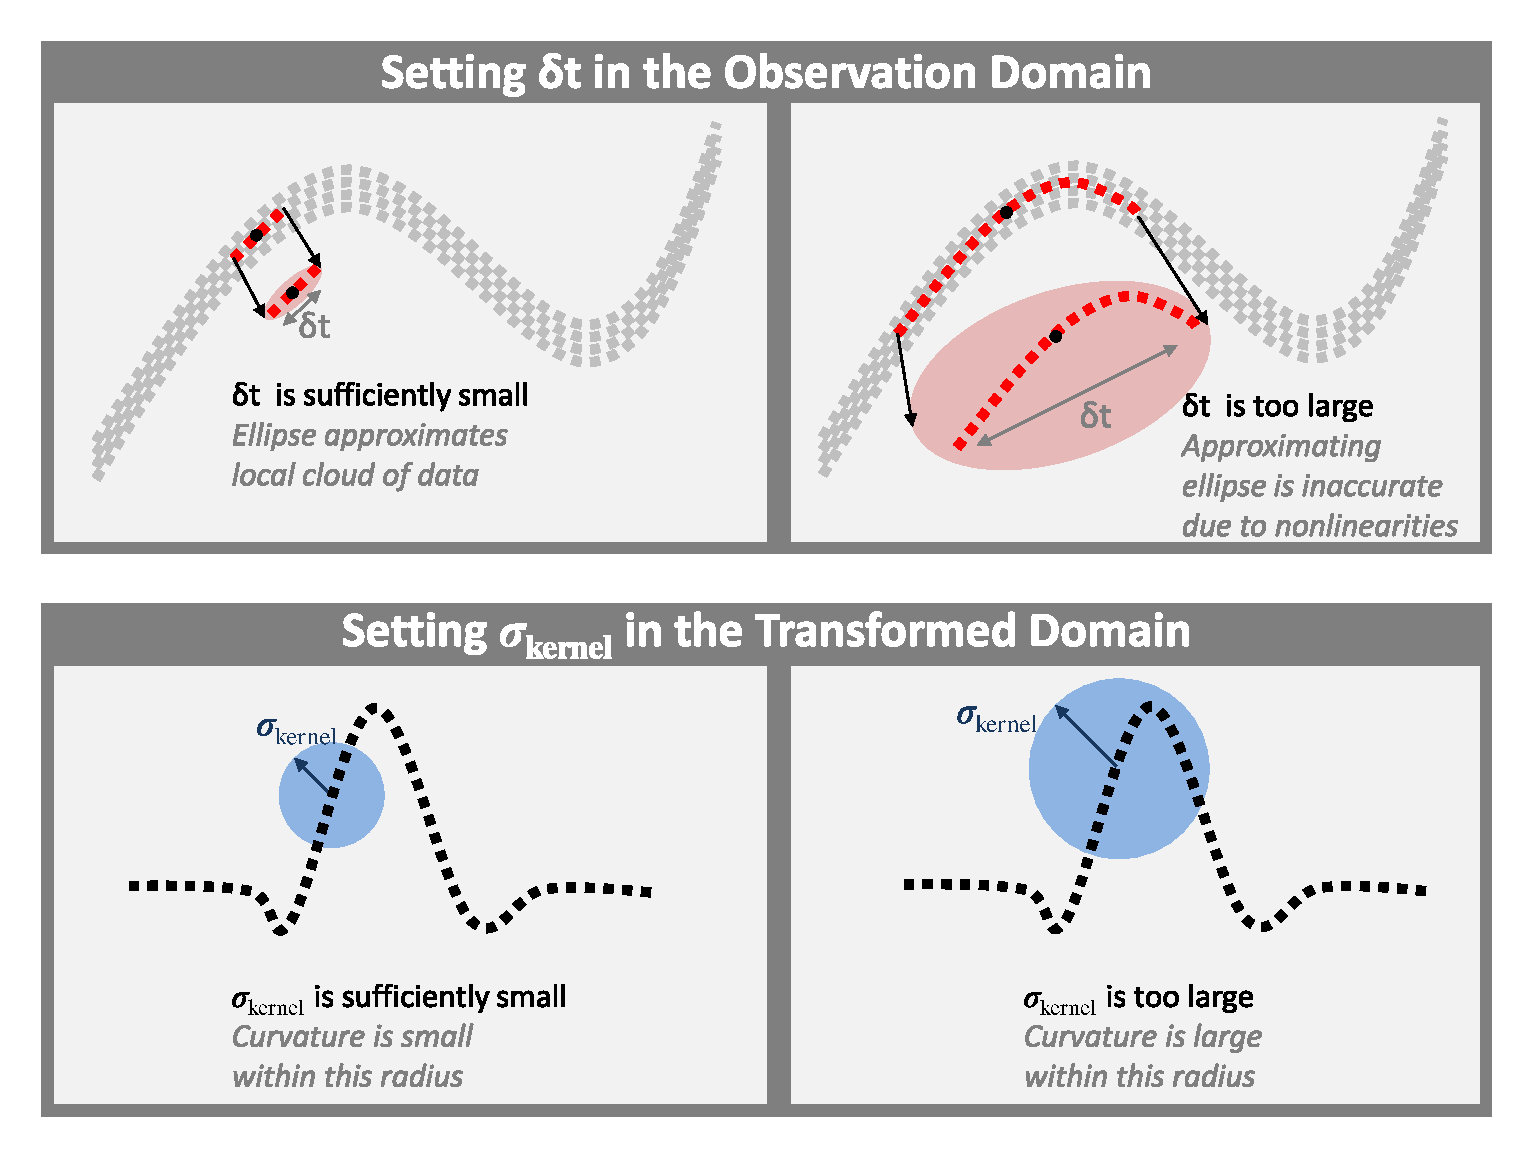
\epsfig{width=\textwidth, file=schematic.eps}
\caption{Illustration of how to choose $\delta t$ and $\sigma_{kernel}$ appropriately. The data shows the evolution of the ``fast'' variable at a fixed value of the ``slow'' variable.  We must choose both parameters so that the curvature effects and other nonlinearities are negligible. }
\label{fig:schematic}
\end{figure}

The traditional Mahalanobis distance is defined for a fixed distribution, whereas we are dealing with a distribution that possibly changes because of any non-linearities in the observation function $\mathbf{f}$ and in the drift $a(\vec{x})$. Consequently we use the following modified definition for the Mahalanobis distance between two points
\begin{equation} \label{eq:mahalanobis_distance}
 \| \vec{y}_2 - \vec{y}_1 \|^2_M =
 \frac{1}{2} (\vec{y}_2 - \vec{y}_1)^T \left( C^{\dagger}(\vec{y}_1) + C^{\dagger}(\vec{y}_2) \right) (\vec{y}_2 - \vec{y}_1)
 \end{equation}
where $C(\vec{y}(t))$ is the covariance of the observed stochastic process at the point $\vec{y}(t)$, $\dagger$ denotes the Moose-Penrose pseudoinverse (since $d$ may exceed $n$).

In the simple case, that $\mathbf{f} (\vec{x}) = A \vec{x}$, the covariance of the accessible sample is given by $C_y=AC_xA^T$. Let $A=U \Lambda V^T$ be the singular value decomposition (SVD) of $A$, where TODO. By the SVD, the pseudoinverse of the covariance matrix is $C^{\dagger}_y = U \Lambda^{-1} V^T C_x^{-1} V \Lambda ^{-1} U^T$. Consequently, the Mahalanobis distance \eqref{eq:mahalanobis_distance} is reduced to
\begin{align} 
\| \vec{y}_2 - \vec{y}_1 \|^2_M &= (\vec{y}_2 - \vec{y}_1)^T  C^{\dagger}_y  (\vec{y}_2 - \vec{y}_1) \\
 &= (\vec{x}_2 - \vec{x}_1)^T A^T C^{\dagger}_y A (\vec{x}_2 - \vec{x}_1) \\
 &= (\vec{x}_2 - \vec{x}_1)^T V \Lambda U^T  U \Lambda^{-1} V^T C_x^{-1} V \Lambda ^{-1} U^T U \Lambda V^T (\vec{x}_2 - \vec{x}_1) \\
 &= (\vec{x}_2 - \vec{x}_1)^T C_x^{-1}  (\vec{x}_2 - \vec{x}_1) \\
 &= \| \vec{x}_2 - \vec{x}_1 \|^2_M =  \| \vec{z}_2 - \vec{z}_1 \|^2_2
\end{align} 
Hence evaluating the Mahalanobis distance of the observations $\mathbf{f}(\vec{x})$ using \eqref{eq:mahalanobis_distance} allows us to estimate the Euclidean distances of the rescaled variables $\vec{z}$ (in which the fast coordinated are collapsed).

Following TODO:Amit, we will show via Taylor expansion that the Mahalanobis distance between the observations \eqref{eq:mahalanobis_distance} approximates the Euclidean distance between the rescaled variables for more general observation functions $\mathbf{f}$. 
%Our approximation of the pairwise distances relies on the Taylor expansion of the measurement function $\mathbf{f}$.
%
\eqref{eq:mahalanobis_distance} cannot be evaluated directly since we do not have access to the covariance matrices, so we will instead estimate the covariances directly from data.
%
If we had a set of values $\{\vec{y}(t_i) \}, i = 1, \ldots , q$ where the $\{\vec{y}(t_i)\}$ are drawn from the local
distribution at $\vec{y}(t_0)$ we can estimate the covariance $C(\vec{y}(t_0))$ empirically. 
%
One way to compute this set of points is to run $q$ simulations for a short time, $\delta t$, each starting from $\vec{y}(t_0)$. Alternatively, we can run a single simulation for a time $q \delta t$ starting from $\vec{y}(t_0)$ to compute a time series of
values $\vec{y}(t_i) , i = 1, \ldots , q$ and then estimate the covariance of the increments
$\Delta \vec{y}(t_i) = \vec{y}(t_i) -\vec{y}(t_{i-1})$. It can be shown that if $q \delta t$ is sufficiently small, the errors introduced
are of lower order than needed.

We will address the accuracy of our method from two standpoints: (1) the accuracy of the Taylor expansion, and (2) the accuracy of the covariance estimation.
%
Figure~\ref{fig:schematic} illustrates some of the issues in choosing the sizes $\delta t$ (or $q \delta t$ if the alternate method is used) and the parameter $\sigma_{kernel}$.
%
We will present both analytical results for the error bounds, as well as an empirical methodology to set the appropriate parameters for our method to accurately recover the slow variable(s).

\subsection{Error analysis of the Mahalanobis distance}

We want to calculate the distance $\|\vec{z}(t_2) - \vec{z}(t_1)\|_2$ in terms of the observations $\vec{y}(t) = \mathbf{f}(\vec{x}(t))$.
%
Let $\mathbf{g} = \mathbf{f}^{-1}: \mathbb{R}^d \mapsto \mathbb{R}^n$, such that
\begin{equation} \label{eq:variable_rescaling}
\sqrt{e_i} g_i(\vec{y}(t)) = \sqrt{e_i} x_i(t) = z_i(t)
\end{equation}
%
By Taylor expansion of $\mathbf{g}(y)$ around $\vec{y}(t_1)$ and $\vec{y}(t_2)$ and averaging the two expansions,
%
\begin{equation} \label{eq:distance_taylor_expansion}
\begin{aligned}
\| \vec{z}(t_2) - \vec{z}(t_1) \|^2_2 =&
\frac{1}{2} \left(\vec{y}(t_2)-\vec{y}(t_1)\right)^T \left(C^\dagger (\vec{y}(t_1)) + C^\dagger (\vec{y}(t_2)) \right) (\vec{y}(t_2)-\vec{y}(t_1)) \\
&+ E_M \left(\vec{y}(t_1), \vec{y}(t_2) \right) \\
&+ \mathcal{O} \left(\| \vec{y}(t_2) - \vec{y}(t_1) \|^6_2 \right)
\end{aligned}
\end{equation}
 and $E_M$ is a fourth-order error term.
%
Because we can empirically estimate $C(\vec{y}(t))$ from data (this will be discussed in Section~\ref{subsec:cov_est}), we choose to truncate the distance approximation in \eqref{eq:distance_taylor_expansion} at the second order term;
we call this distance the Mahalanobis distance \footnote{We would like to note that the Mahalanobis distance is traditionally defined for a fixed covariance matrix. However, following \cite{...}, we will define our Mahalanobis distance locally, using the local covariance at each point.},










%
The error incurred by using the Mahalanobis distance to approximate the true distance between points, $E_M$, can be shown to be
%
\begin{equation}
\begin{aligned} \label{eq:mahanaobis_error}
E_M\left( \vec{y}(t_1), \vec{y}(t_2) \right)
 =
\frac{1}{2} \sum_{i=1}^n \sum_{jkl=1}^{d} &
\left( g_{i, (j)} (\vec{y}(t_1)) g_{i, (k,l)} (\vec{y}(t_1)) -  g_{i, (j)} (\vec{y}(t_2)) g_{i, (k,l)} (\vec{y}(t_2)) \right) \\
& (\vec{y}_j(t_2) - \vec{y}_j(t_1))   (\vec{y}_k(t_2) - \vec{y}_k(t_1))(\vec{y}_l(t_2) - \vec{y}_l(t_1)) \\
+ \frac{1}{8} \sum_{i=1}^n \sum_{jklm=1}^d  &
\left( g_{i, (j,k)} (\vec{y}(t_1)) g_{i, (l,m)} (\vec{y}(t_1)) +  g_{i, (j,k)} (\vec{y}(t_2)) g_{i, (l,m)} (\vec{y}(t_2)) \right) \\
&(\vec{y}_j(t_2) - \vec{y}_j(t_1))  (\vec{y}_k(t_2) - \vec{y}_k(t_1))(\vec{y}_l(t_2) - \vec{y}_l(t_1)) (\vec{y}_m(t_2) - \vec{y}_m(t_1)) \\
+ \frac{1}{6} \sum_{i=1}^n \sum_{jklm=1}^d &
\left( g_{i, (j)} (\vec{y}(t_1)) g_{i, (k,l,m)} (\vec{y}(t_1)) +  g_{i, (j)} (\vec{y}(t_2)) g_{i, (k,l,m)} (\vec{y}(t_2)) \right) \\
& (\vec{y}_j(t_2) - \vec{y}_j(t_1))  (\vec{y}_k(t_2) - \vec{y}_k(t_1))(\vec{y}_l(t_2) - \vec{y}_l(t_1))(\vec{y}_m(t_2) - \vec{y}_m(t_1))
\end{aligned}
\end{equation}
%
where
%
\begin{equation}
\begin{aligned}
g_{i,(j)} &= \sqrt{e_i} \frac{\partial g_i}{\partial y_j}
\\
g_{i,(j,k)} &= \sqrt{e_i}  \frac{\partial^2 g_i}{\partial y_j \partial y_k}
\\
g_{i,(j,k,l)} &= \sqrt{e_i}  \frac{\partial^3 g_i}{\partial y_j \partial y_k \partial y_l}
\end{aligned}
\end{equation}
%
%% original expansion before changing derivative notation
%{\small
%\begin{equation} \label{eq:distance_taylor_expansion}
%\begin{aligned}
%&\| \vec{z}_2 - \vec{z}_1 \|^2_2 = \\
%& \frac{1}{2} \sum_{i=1}^n \sum_{jk=1}^d e_i \left( \left. \frac{\partial g_i}{\partial y_j} \right|_{\vec{y}_1} \left. \frac{\partial g_i}{\partial y_k} \right|_{\vec{y}_1} + \left. \frac{\partial g_i}{\partial y_j} \right|_{\vec{y}_2} \left. \frac{\partial g_i}{\partial y_k } \right|_{\vec{y}_2} \right) (y_{2,j} - y_{1,j}) (y_{2,k} - y_{1,k}) \\
%& + \frac{1}{2} \sum_{i=1}^n \sum_{jkl=1}^{d} e_i \left( \left. \frac{\partial g_i}{\partial y_j} \right|_{\vec{y}_1} \left. \frac{\partial^2 g_i}{\partial y_k \partial y_l} \right|_{\vec{y}_1} - \left. \frac{\partial g_i}{\partial y_j} \right|_{\vec{y}_2} \left. \frac{\partial^2 g_i}{\partial y_k \partial y_l} \right|_{\vec{y}_2} \right) (y_{2,j} - y_{1,j})  (y_{2,k} - y_{1,k})(y_{2,l} - y_{1,l}) \\
%& + \frac{1}{8} \sum_{i=1}^n \sum_{jklm=1}^d  e_i \left( \left. \frac{\partial^2 g_i}{\partial y_j \partial y_k} \right|_{\vec{y}_1} \left. \frac{\partial^2 g_i}{\partial y_l \partial y_m} \right|_{\vec{y}_1} + \left. \frac{\partial^2 g_i}{\partial y_j \partial y_k} \right|_{\vec{y}_2} \left. \frac{\partial^2 g_i}{\partial y_l \partial y_m} \right|_{\vec{y}_2} \right) (y_{2,j} - y_{1,j})  (y_{2,k} - y_{1,k})(y_{2,l} - y_{1,l})(y_{2,m} - y_{1,m}) \\
%& + \frac{1}{6} \sum_{i=1}^n \sum_{jklm=1}^d e_i \left( \left. \frac{\partial g_i}{\partial y_j} \right|_{\vec{y}_1} \left. \frac{\partial^3 g_i}{ \partial y_k \partial y_l \partial y_m} \right|_{\vec{y}_1} + \left. \frac{\partial g_i}{\partial y_j} \right|_{\vec{y}_2} \left. \frac{\partial^3 g_i}{ \partial y_k \partial y_l \partial y_m} \right|_{\vec{y}_2} \right) (y_{2,j} - y_{1,j})  (y_{2,k} - y_{1,k})(y_{2,l} - y_{1,l})(y_{2,m} - y_{1,m}) \\
%& + \mathcal{O} (\|\vec{y}_1 - \vec{y}_2 \|^6 ),
%\end{aligned}
%\end{equation}
%}
%
From this expression, the error incurred by using the Mahalanobis distance to approximate the $L_2$-distance between points $\vec{z}(t)$ is a function of the second- and higher-order derivatives of $\mathbf{g}$, as well as the distance between samples $\| \vec{y}(t_2) - \vec{y}(t_1) \|_2$.
%
The parameter $\sigma_{kernel}$ in the diffusion maps calculation determines how much $E_M$ contributes to the overall analysis.
%
From \eqref{eq:dmaps_kernel}, distances which are greater than $\sigma_{kernel}$ are ``not important'' in the computation because of the exponential kernel.
%
Therefore, we want to choose $\sigma_{kernel}^2$ on the order of $\|\vec{y}(t_2) - \vec{y}(t_1)\|^2$ in a regime where $E_M(\vec{y}(t_1), \vec{y}(t_2)) \ll \|\vec{y}(t_2) - \vec{y}(t_1)\|^2$.
%
This is illustrated in Figure~\ref{fig:schematic}, where we want to choose $\sigma_{kernel}$ small enough so that the curvature and other nonlinear effects (captured in the error term $E_M$) are negligible.
%
This will ensure that the errors in the Mahalanobis distance approximation do not greatly effect our overall analysis.

\subsection{Error analysis of the covariance estimation} \label{subsec:cov_est}

To compute the Mahalanobis distance in \eqref{eq:mahalanobis_distance}, we require $C$, the covariance of the observed stochastic process.
%
We will use simulation bursts to estimate the covariance at a point $\vec{y}(t)$ from data.
%
Let $\vec{y}(t)$ be the point at which  we want to estimate the covariance.
%
We then write the estimated covariance $\hat{C}(\vec{y}(t), \delta t)$, as
\begin{equation}\label{eq:estimated_cov_expected_value}
\hat{C}_{ij}(\vec{y}(t), \delta t)
=
\frac{1}{\delta t} \left( \mathbb{E} \left[ y_i (t+\delta t) y_j (t+ \delta t) \mid \vec{y}(t) \right]
- \mathbb{E} \left[ y_i (t+\delta t) \mid \vec{y}(t) \right] \mathbb{E} \left[ y_j (t+\delta t) \mid \vec{y}(t) \right] \right)
\end{equation}
%
where $\delta t > 0$ is the length of the simulation burst.

We know that, for a stochastic process following \eqref{eq:general_SDE} and observed through a function $\mathbf{f}$, the covariance $C$ is given by
\begin{equation} \label{eq:analytical_cov}
C_{ij}(\vec{y}(t)) =
\sum_{k=1}^n \frac{1}{e_k} \left. \frac{\partial f_{i}}{\partial x_k} \right|_{\vec{x}(t)} \left. \frac{\partial f_{j}}{\partial x_k} \right|_{\vec{x}(t)}
\end{equation}
%
By It\={o}-Taylor expansion of $\mathbf{f}$ and $\vec{x}(t)$,
\begin{equation}\label{eq:estimated_cov}
\begin{aligned}
\hat{C}_{ij} (\vec{x}_t, \delta t)
=&
\frac{1}{\delta t} \left( \mathbb{E} \left[ y_i (t+\delta t) y_j (t+ \delta t) \mid \vec{y}(t) \right]
- \mathbb{E} \left[ y_i (t+\delta t) \mid \vec{y}(t) \right] \mathbb{E} \left[ y_j (t+\delta t) \mid \vec{y}(t) \right] \right)
\\
=& \sum_{k=1}^n \frac{1}{e_k} \left. \frac{\partial f_{i}}{\partial x_k} \right|_{\vec{x}(t)} \left. \frac{\partial f_{j}}{\partial x_k} \right|_{\vec{x}(t)}
+ E_{C, ij} (\vec{x}(t), \delta t) + \mathcal{O}(\delta t^{3/2})
%=& \sum_{k=1}^n \frac{1}{e_k} \left. \frac{\partial f_{i}}{\partial x_k} \right|_{\vec{x}(t)} \left. \frac{\partial f_{j}}{\partial x_k} \right|_{\vec{x}(t)} \\
%&+ \frac{1}{\delta t} \sum_{k=1}^n f_{i,(k)}(\vec{x}(t)) \left( \mathbb{E} \left[ \int_t^{t+\delta t} \int_{s_1}^{t+\delta t} f_{j,(k,0)}(\vec{x}(s_2)) ds_2 ds_1 \right]
%+ \mathbb{E} \left[  \int_t^{t+\delta t} \int_t^{s_2} f_{j,(0,k)}(\vec{x}(s_1)) ds_1 ds_2\right] \right) \\
%&+  \frac{1}{\delta t} \sum_{k=1}^n f_{j,(k)}(\vec{x}(t)) \left( \mathbb{E} \left[ \int_t^{t+\delta t} \int_{s_1}^{t + \delta t} f_{i,(k,0)}(\vec{x}(s_2)) ds_2 ds_1 \right]
%+ \mathbb{E} \left[ \int_t^{t+\delta t} \int_t^{s_2} f_{i,(0,k)}(\vec{x}(s_1)) ds_1 ds_2 \right] \right) \\
%&+  \frac{1}{\delta t} \sum_{k,l=1}^n \mathbb{E} \left[ \int_t^{t+\delta t}\left( \int_t^{s_2} f_{i,(k,l)}(\vec{x}(s_1)) dW_{s_1, k}  \right) \left(  \int_t^{s_2} f_{j,(k,l)}(\vec{x}(s_1)) dW_{s_1, k} \right) ds_2 \right] \\
%&+ \mathcal{O} (\delta t^{3/2}),
\end{aligned}
\end{equation}
%
where $E_C = \mathcal{O} (\delta t)$ is an error term, with
%
\begin{equation} \label{eq:cov_error}
\begin{aligned}
E_{C, ij} (\vec{x}(t), \delta t) =&
 \frac{1}{\delta t} \sum_{k=1}^n f_{i,(k)}(\vec{x}(t)) \mathbb{E} \left[ \int_t^{t+\delta t} \left( \int_{s_2}^{t+\delta t} f_{j,(k,0)}(\vec{x}(s_1)) ds_1
+ \int_t^{s_2} f_{j,(0,k)}(\vec{x}(s_1)) ds_1 \right) ds_2 \right] \\
&+  \frac{1}{\delta t} \sum_{k=1}^n f_{j,(k)}(\vec{x}(t))  \mathbb{E} \left[ \int_t^{t+\delta t} \left( \int_{s_2}^{t + \delta t} f_{i,(k,0)}(\vec{x}(s_1)) ds_1
+  \int_t^{s_2} f_{i,(0,k)}(\vec{x}(s_1)) ds_1 \right) ds_2 \right] \\
&+  \frac{1}{\delta t} \sum_{k,l=1}^n \mathbb{E} \left[ \int_t^{t+\delta t}\left( \int_t^{s_2} f_{i,(k,l)}(\vec{x}(s_1)) dW_{s_1, k}  \right) \left(  \int_t^{s_2} f_{j,(k,l)}(\vec{x}(s_1)) dW_{s_1, k} \right) ds_2 \right]
\end{aligned}
\end{equation}
%
where
\begin{equation}
\begin{aligned}
f_{i,(k)} &= \frac{1}{\sqrt{e_k}} \frac{\partial f_i}{\partial x_k}
\\
f_{i,(k,l)} &= \frac{1}{\sqrt{e_k e_l}} \frac{\partial^2 f_i}{\partial x_k \partial x_l}
\\
f_{i,(k,0)} &= \frac{1}{\sqrt{e_k}} \sum_{l=1}^n \left( \frac{\partial}{\partial x_k} \left( \frac{a_l(\vec{x})}{e_l} \frac{\partial f_i}{\partial x_l} \right) + \frac{1}{2 e_l} \frac{\partial^3 f_i}{\partial x_k \partial x_l^2} \right)
\\
f_{i,(0, k)} &= \frac{1}{\sqrt{e_k}} \sum_{l=1}^n \left( \frac{a_l(\vec{x})}{e_l} \frac{\partial^2 f_i}{\partial x_k \partial x_l} +\frac{1}{2 e_l}  \frac{\partial^3 f_i}{\partial x_k \partial^2 x_l} \right).
\end{aligned}
\end{equation}
%
From \eqref{eq:cov_error}, the error in the covariance is a function of the derivatives of $\mathbf{f}$ and $\mathbf{a}$, as well as $\delta t$.
%
We want to set $\delta t$ such that $\|E_C \| \ll \|C \|$
(this is illustrated in Figure~\ref{fig:schematic}).
%
In practice, we compute $\hat{C}$ by running many simulations of length $\delta t$ starting from $\vec{x}(t)$, and using the sample average to approximate the expected values in \eqref{eq:estimated_cov_expected_value}.

\section{Results}

For illustrative purposes, we will consider the following two-dimensional SDE as a specific example of \eqref{eq:general_SDE},
\begin{equation} \label{eq:specific_SDE}
\begin{aligned}
dx_1(t) &=& adt &+& dW_1(t)\\
dx_2(t) &=& -\frac{x_2(t)}{\epsilon} dt &+& \frac{1}{\sqrt{\epsilon}} dW_2(t)
\end{aligned}
\end{equation}
%
where $a$ is a constant of order 1.
%
$x_1$ is the slow variable, and $x_2$ is a fast noise whose equilibrium measure is bounded and $\mathcal{O}(1)$.
%
Figure~\ref{fig:initial_data} shows data simulated from this SDE, colored by time.
%
We would like to recover a parametrization of this data that is one-to-one with the slow variable $x_1$.

\begin{figure}[t]
\centering
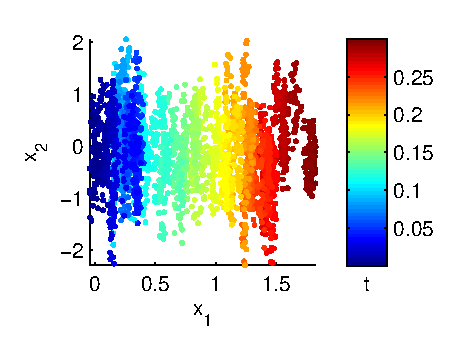
\epsfig{width=0.5\textwidth, file=data_init.eps}

\vspace{0.25in}
\caption{Data, simulated from \eqref{eq:specific_SDE} with $a=3$ and $\epsilon = 10^{-3}$, for $3000$ time steps with $dt = 10^{-4}$. The data are colored by time.}
\label{fig:initial_data}
\end{figure}

\subsection{Linear functions} \label{subsec:linear_example}

In the first example, our observation function $\mathbf{f}$ will be the identity function,
%
\begin{equation} \label{eq:linear_transform}
\begin{aligned}
\begin{bmatrix}
y_1(t) \\ y_2(t)
\end{bmatrix} &=&
\mathbf{f}(\vec{x}(t)) &=&
\begin{bmatrix} x_1(t) \\ x_2(t) \end{bmatrix} \\
\mathbf{g}(\vec{y}(t)) &=& \mathbf{f}^{-1} (\vec{y}(t)) &=& \begin{bmatrix} y_1(t) \\ y_2(t) \end{bmatrix}
\end{aligned}
\end{equation}
%
where the fast and slow variables remain uncoupled.
%
In this case, $E_M = 0$, as the second- and higher-order derivatives of $\mathbf{g}$ are identically 0.

\subsubsection{Importance of using the Mahalanobis distance}

We first want to demonstrate the utility of using the Mahalanobis distance compared to the typical Euclidean distance.
%
We compute the diffusion maps embedding for the data in Figure~\ref{fig:initial_data}, using both the Mahalanobis distance and the Euclidean distance for the computation of the kernel in \eqref{eq:dmaps_kernel}.
%
The data, colored by $\phi_1$ using the two different metrics, are shown in Figure~\ref{fig:NIV_versus_DMAPS}.
%
Using the Mahalanobis distance allows us to accurately recover the slow variable, as the coloring in Figure~\ref{fig:NIV_versus_DMAPS}(a) is consistent with the coloring in Figure~\ref{fig:initial_data}.
%
In contrast, using the Euclidean distance does not allow us recover the slow variable using diffusion maps.

\begin{figure}[t]
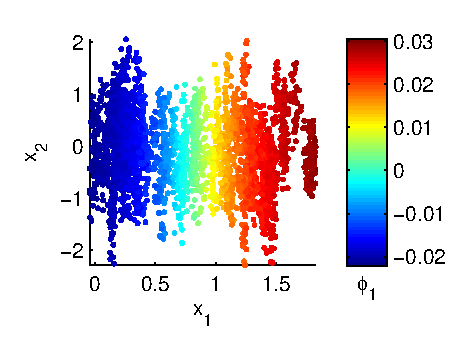
\epsfig{width=0.5\textwidth, file=data_linear_NIV.eps}
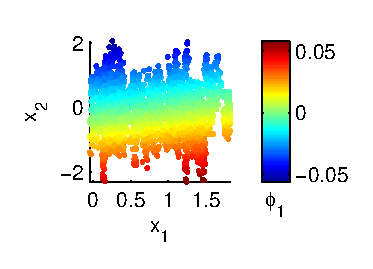
\epsfig{width=0.5\textwidth, file=data_linear_DMAPS.eps}

\vspace{0.25in}
\hspace{0.2\textwidth}
(a)
\hspace{0.45\textwidth}
(b)

\caption{Comparison of using the Mahalanobis distance and the Euclidean distance. (a) The data from Figure~\ref{fig:initial_data}, colored by the first diffusion maps coordinate when using the Mahalanobis distance in the kernel. (b) The data from Figure~\ref{fig:initial_data}, colored by the first diffusion maps coordinate when using the Euclidean distance in the kernel. Note that we do {\em not} recover the slow variable.}
\label{fig:NIV_versus_DMAPS}
\end{figure}

\subsubsection{Errors in covariance estimation}

For the example in \eqref{eq:linear_transform}, the analytical covariance is
 \begin{equation} \label{eq:cov_linear_example}
C(\vec{x}(t)) =
\begin{bmatrix}
1 & 0 \\
0 & \frac{1}{\epsilon}
\end{bmatrix}.
\end{equation}
%
From \eqref{eq:estimated_cov}, we find
%
\begin{equation}
E_C(\vec{x}(t), \delta t) =
\begin{bmatrix}
0 & 0 \\
0 & -\frac{\delta t}{\epsilon^2}
\end{bmatrix}
\end{equation}
%
Therefore, $\| C \| = \mathcal{O} \left( \frac{1}{\epsilon} \right)$ and $\|E_C \| = \mathcal{O}\left(\frac{\delta t}{\epsilon^2} \right)$.
%
These terms are shown in Figure~\ref{fig:cov_error}(a) as a function of $\delta t$.
%
We want to choose $\delta t$ in a regime where $\| E_c \| \ll \| C\|$, so that the errors in the estimated covariance are small.

When we do not analytically know the functions $\mathbf{f}$ or $\mathbf{g}$, we can find such a regime empirically by
estimating the covariance for several values of $\delta t$.
%
This will provide an estimate of $\hat{C} = C + E_C$ as a function of $\delta t$.
%
From Figure~\ref{fig:cov_error}(a), we can see that there should be a kink in the plot of $\| \hat{C} \|$ versus $\delta t$ when $\| E_C \|$ becomes larger than $\|C\|$.
%
Figure~\ref{fig:cov_error}(b) shows the empirical $\| \hat{C} \|$ as a function of $\delta t$, and the kink in this curve is consistent with the crossover point in Figure~\ref{fig:cov_error}(a).

\begin{figure}[t]
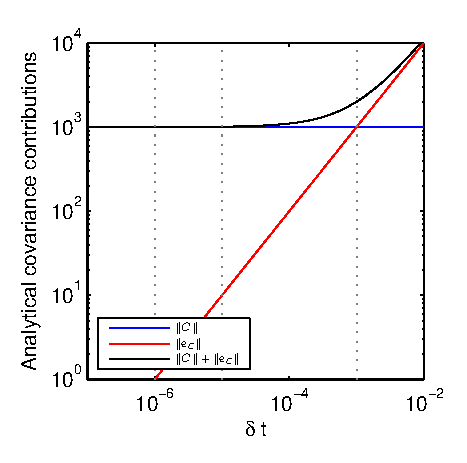
\epsfig{width=0.5\textwidth, file=C_dt_analytical_linear.eps}
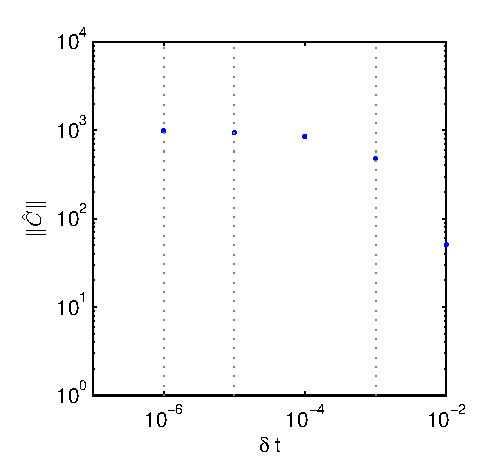
\epsfig{width=0.5\textwidth, file=C_dt_linear.eps}

\hspace{0.25\textwidth}
(a)
\hspace{0.45\textwidth}
(b)

\caption{Errors in covariance estimation for linear example. (a) The analytical expressions for the contributions to the covariance for the example in Section~\ref{subsec:linear_example} as a function of $\delta t$. (b) The average estimated covariance $\| \hat{C} \|$ as a function of $\delta t$. The average is computed over $10$ test points and using $50$ sample points to estimate the covariance.}
\label{fig:cov_error}
\end{figure}

\subsubsection{Recovery of fast variable}

Note that, for this linear example, $E_C$ is a constant diagonal matrix.
%
Therefore, taking $\delta t$ ``too large'' will not lead to nonlinear effects or mixing of the fast and slow variables. %
Rather, changing $\delta t$ will only affect the perceived ratio of the fast and slow timescales.
%
Figure~\ref{fig:recover_fast} shows results for three different values of $\delta t$ (the corresponding values are indicated by the dashed lines on Figure~\ref{fig:cov_error}).
%
When the time scale of the simulation burst used to estimate the local covariance (indicated by the red clouds in the top row of figures) is shorter than that of the equilibration time of the fast variable, the estimated covariance is constant and the fast variable is collapsed significantly relative to the slow variable.
%
This means that the fast variable is recovered {\em very} far down in the diffusion maps eigenvectors.
%
The left two columns of Figure~\ref{fig:recover_fast} show that, for this example, when the simulation burst is shorter than the equilibration time, the fast variable is recovered as $\phi_{10}$.
%
However, if the time scale of the burst is {\em longer} than the saturation time of the fast variable, the estimated covariance changes: the variance in the slow direction continues to grow, while the variance in the fast direction is fixed.
%
This means that the collapse of the fast variable is less pronounced relative to the slow variable, and the fast variable is recovered in a higher eigenvector.
%
The right column of Figure~\ref{fig:recover_fast} shows that, when the burst is now longer than the equilibration time, the fast variable appears higher in the eigenvalue spectrum and is recovered as $\phi_6$.

\begin{figure}[t]
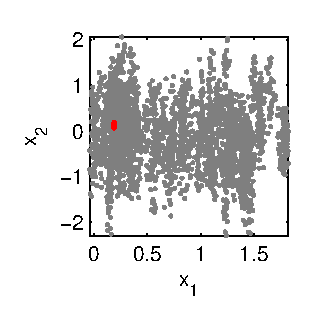
\epsfig{width=0.3\textwidth, file=data_linear_burst1.eps}
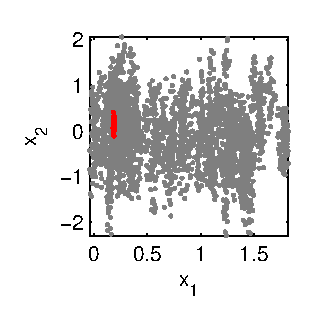
\epsfig{width=0.3\textwidth, file=data_linear_burst2.eps}
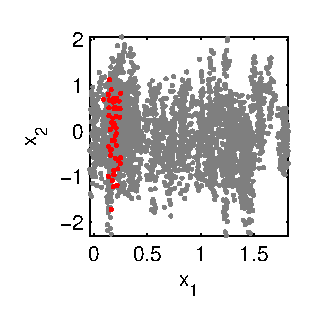
\epsfig{width=0.3\textwidth, file=data_linear_burst3.eps}

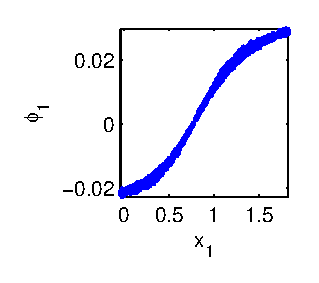
\epsfig{width=0.3\textwidth, file=data_linear_slow1.eps}
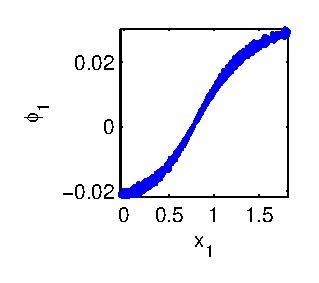
\epsfig{width=0.3\textwidth, file=data_linear_slow2.eps}
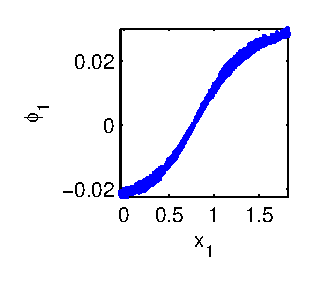
\epsfig{width=0.3\textwidth, file=data_linear_slow3.eps}

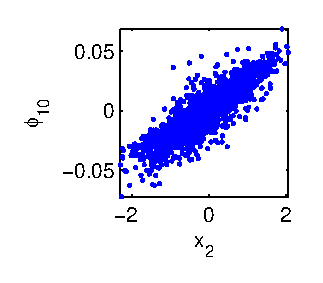
\epsfig{width=0.3\textwidth, file=data_linear_fast1.eps}
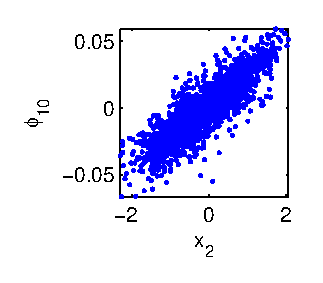
\epsfig{width=0.3\textwidth, file=data_linear_fast2.eps}
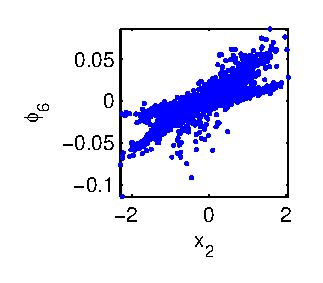
\epsfig{width=0.3\textwidth, file=data_linear_fast3.eps}

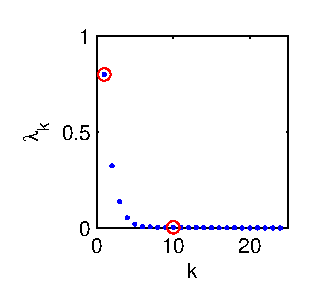
\epsfig{width=0.3\textwidth, file=data_linear_evals1.eps}
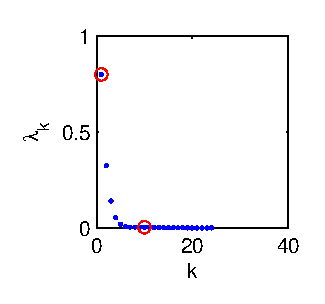
\epsfig{width=0.3\textwidth, file=data_linear_evals2.eps}
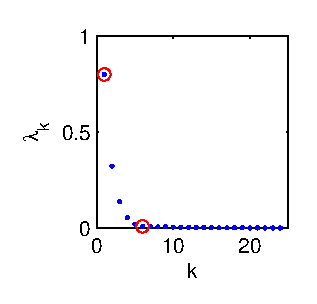
\epsfig{width=0.3\textwidth, file=data_linear_evals3.eps}

\caption{Relationship between changing $\delta t$ and recovery of the variables. From left to right, the columns correspond to $\delta t = 10^{-6}, 10^{-5}, 10^{-3}$.  (Row 1) Data (gray) and representative burst (red) used to estimate the local covariance. (Row 2) Correlation between first diffusion maps coordinate and the slow variable $x_1$. (Row 3) Correlation between diffusion maps coordinate and the fast variable $x_2$. Note that for $\delta t = 10^{-6}, 10^{-5}$, $x_2$ is correlated with $\phi_{10}$, whereas when $\delta t = 10^{-3}$, $x_2$ is correlated with $\phi_6$. (Row 4) Diffusion maps eigenvalue spectra. The eigenvalues corresponding to the coordinates for the fast and slow modes are indicated by red circles. }
\label{fig:recover_fast}
\end{figure}

\subsection{Nonlinear functions} \label{subsec:nonlinear_example}

In the second example, our data will be warped into half-moon shapes via the function
\begin{equation} \label{eq:nonlinear_function}
\begin{aligned}
\begin{bmatrix}
y_1(t) \\ y_2(t)
\end{bmatrix} &=&
\mathbf{f}(\vec{x}(t)) &=&
\begin{bmatrix}
x_1(t) + x_2^2(t) \\
x_2(t)
\end{bmatrix}\\
\mathbf{g}(\vec{y}(t)) &=& \mathbf{f}^{-1} (\vec{y}(t)) &=& \begin{bmatrix} y_1(t) - y_2^2(t) \\ y_2(t) \end{bmatrix}
\end{aligned}
\end{equation}
%
Figure~\ref{fig:initial_data_nonlinear} shows the data from Figure~\ref{fig:initial_data} transformed by the function $\mathbf{f}$ and colored by time.
%
For this example, the analytical covariance and inverse covariance are
\begin{equation}
\begin{aligned}
C(\vec{x}(t)) =&
\frac{1}{\epsilon}
 \begin{bmatrix}
\epsilon + 4x_2^2(t) & 2x_2(t) \\
2x_2(t) & 1
\end{bmatrix}\\
C^{\dagger}(\vec{x}(t)) =&
\begin{bmatrix}
1 & -2 x_2(t) \\
-2 x_2(t) & \epsilon+ 4 x_2^2(t)
\end{bmatrix}
\end{aligned}
\end{equation}

The fast and slow variables are now mixed through the function $\mathbf{f}$, and so the Euclidean distance is not informative about the fast {\em or} the slow variables.
%
Figure~\ref{fig:colored_data_nonlinear_cases}(b) shows the data from Figure~\ref{fig:initial_data_nonlinear}, colored by the first diffusion maps coordinate computed using the Euclidean distance between data points.
%
Clearly, this coordinate is not informative about the slow (or the fast) variable in the data, and we need to use the Mahalanobis distance to obtain a parametrization that is consistent with the underlying dynamics.
%
Figure~\ref{fig:colored_data_nonlinear_cases}(a) shows the data from Figure~\ref{fig:initial_data_nonlinear}, colored by the first diffusion maps coordinate computed using the Mahalanobis distance between data points.
%
We now successfully recover the slow variable.

\begin{figure}[t]
\centering
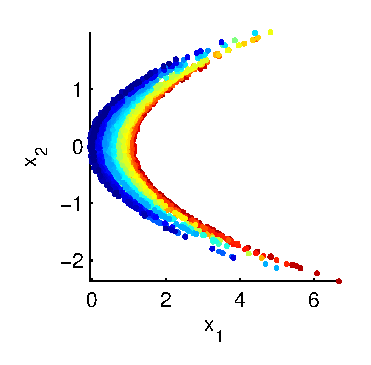
\epsfig{width=0.5\textwidth, file=data_init_nonlinear.eps}

\vspace{0.25in}
\caption{The data from Figure~\ref{fig:initial_data}, transformed by $\mathbf{f}$ in \eqref{eq:nonlinear_function}}
\label{fig:initial_data_nonlinear}
\end{figure}

\subsubsection{Errors in Mahalanobis distance}

We can bound the Mahalanobis distance by the eigenvalues of $C^{\dagger}$,
\begin{equation}
\lambda_{C^{\dagger},1} \| \vec{y}(t_2) - \vec{y}(t_1) \|_2^2
\le
\| \vec{y}(t_2) - \vec{y}(t_1) \|^2_M
\le
\lambda_{C^{\dagger},2} \| \vec{y}(t_2) - \vec{y}(t_1) \|_2^2
\end{equation}
where $\lambda_{C^{\dagger},1} \le \lambda_{C^{\dagger},2}$ are the two eigenvalues of $C^{\dagger}$.
%
For the example in \eqref{eq:nonlinear_function}, we have
\begin{equation}
E_M(\vec{y}(t_1), \vec{y}(t_2)) = - (y_2(t_2) - y_2(t_1))^4
\end{equation}

Figure~\ref{fig:cov_error_nonlinear}(a) shows $\| \vec{y}(t_2) - \vec{y}(t_1) \|^2_M$ and $E_M$ as a function of $\| \vec{y}(t_2) - \vec{y}(t_1) \|_2$.
%
The Mahalanobis distance is an accurate approximation to the true intrinsic distance $\| \vec{z}(t_2) - \vec{z}(t_1) \|_2$ when $E_M \ll \| \vec{y}(t_2) - \vec{y}(t_1) \|^2_M$.
%
We want to choose $\sigma_{kernel}^2$ in a regime where $E_M(\vec{y}(t_1), \vec{y}(t_2)) \ll \| \vec{y}(t_2) - \vec{y}(t_1) \|^2_M$, so that the distances we utilize in the diffusion maps calculation are accurate.
%
We can find such a regime empirically by plotting $\| \vec{y}(t_2) - \vec{y}(t_1) \|^2_M$ as a function of $\| \vec{y}(t_2) - \vec{y}(t_1) \|_2$, and assessing when the relationship deviates from quadratic.
%
This is shown in Figure~\ref{fig:cov_error_nonlinear}(b), and the deviation from quadratic behavior is consistent with the crossover point in the analytical expressions plotted in Figure~\ref{fig:cov_error_nonlinear}(a).

Figures~\ref{fig:colored_data_nonlinear_cases}(a) and (c) show the data from Figure~\ref{fig:initial_data_nonlinear}, colored by $\phi_1$ for two different values of $\sigma_{kernel}$.
%
The corresponding values of $\sigma_{kernel}^2$ are indicated by the dashed lines in Figure~\ref{fig:cov_error_nonlinear}(a)~and~(b).
%
When $\sigma_{kernel}^2$ corresponds to a region where $\|E_M \| \ll \|\vec{y}(t_2) - \vec{y}(t_1) \|_M^2$, $\phi_1$ is well correlated with the slow variable.
%
However, when $\sigma_{kernel}^2$ corresponds to a region where $\|E_M \| \gg \|\vec{y}(t_2) - \vec{y}(t_1) \|_M^2$, the slow variable is no longer recovered.

\begin{figure}[t]

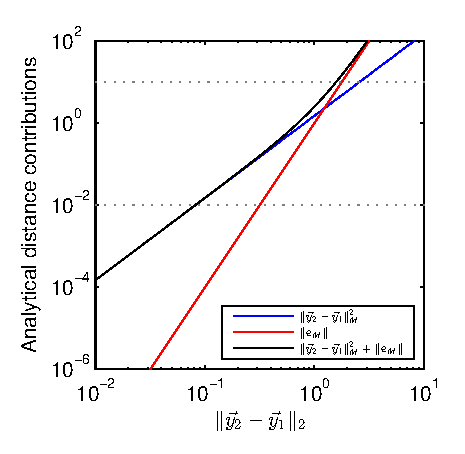
\epsfig{height=3in, file=dist_dy_analytical_nonlinear.eps}
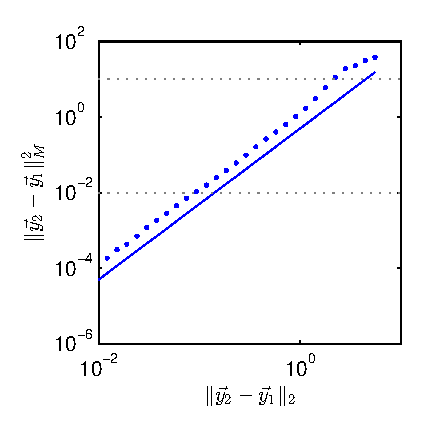
\epsfig{height=3in, file=dist_dy_nonlinear.eps}


\vspace{0.5in}
\hspace{0.25\textwidth}
(a)
\hspace{0.45\textwidth}
(b)

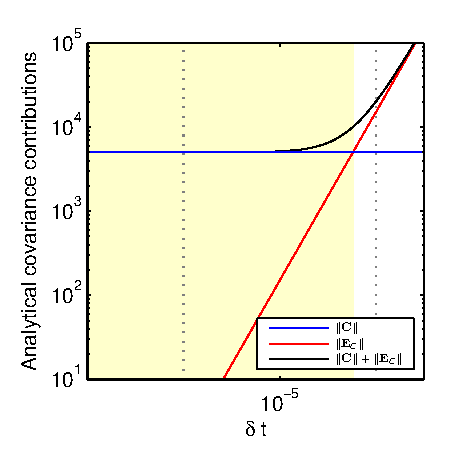
\epsfig{height=3in, file=C_dt_analytical_nonlinear.eps}
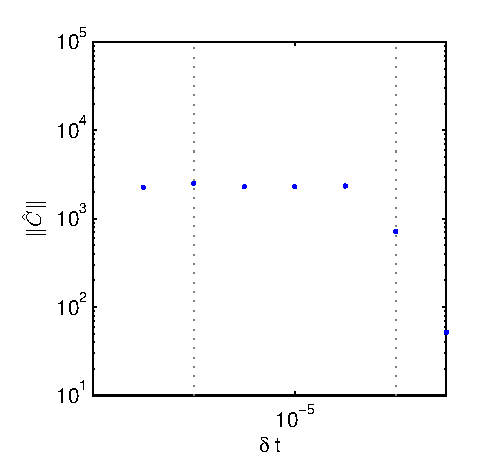
\epsfig{height=3in, file=C_dt_nonlinear.eps}

\hspace{0.25\textwidth}
(c)
\hspace{0.45\textwidth}
(d)

\caption{Errors in the Mahalanobis distance and the covariance estimation for the nonlinear example. (a) The analytical expressions for the contributions to the distance approximation as a function of $\| \vec{y}_2 - \vec{y}_1\|_2$. (b) The average estimated Mahalanobis distance $\| \vec{y}_2 - \vec{y}_1\|^2_M$ as a function of the distance $\| \vec{y}_2 - \vec{y}_1\|_2$. The line $\| \vec{y}_2 - \vec{y}_1\|^2_M = \| \vec{y}_2 - \vec{y}_1\|_2$ is shown for reference. (c) The analytical expressions for the contributions to the covariance as a function of $\delta t$. (d) The average estimated covariance $\| \hat{C} \|$ as a function of $\delta t$. }
\label{fig:cov_error_nonlinear}
\end{figure}

\subsubsection{Errors in covariance estimation}

From \eqref{eq:estimated_cov}, we find that, for the example in \eqref{eq:nonlinear_function},
%
\begin{equation}
\begin{aligned}
E_{C,11} (\vec{x}(t), \delta t)
=&
\frac{2 \delta t}{\epsilon^2}
- \frac{8 x_2(t)}{\epsilon^2 \delta t} \mathbb{E} \left[ \int_t^{t+\delta t} \left( \int_{s_2}^{t+\delta t} 2 x_2(s_1) ds_1
+  \int_t^{s_2} x_2(s_1) ds_1 \right) ds_2\right]  \\
%%
%
E_{C, 12} (\vec{x}(t), \delta t)
=
E_{C, 21} (\vec{x}(t), \delta t)
=&
- \frac{x_2(t) \delta t}{\epsilon^2}
- \frac{2}{\epsilon^2 \delta t} \mathbb{E} \left[ \int_t^{t+\delta t} \left( \int_{s_2}^{t + \delta t} 2 x_2(s_1) ds_1 + \int_t^{s_2} x_2(s_1) ds_1 \right) ds_2 \right] \\
%%
%%
E_{C, 22} (\vec{x}(t), \delta t)
=&
-\frac{\delta t}{\epsilon^2}
\end{aligned}
\end{equation}
%
$\|C \|$ and $\| E_C\|  $ are plotted as a function of $\delta t$ in Figure~\ref{fig:cov_error_nonlinear}(c).
%
As in the previous example, we can empirically find where $\| E_C \| \ll \| C \|$  by plotting $\| \hat{C} \|$ as a function of $\delta t $ and looking for a kink in the plot.
%
These results are shown in Figure~\ref{fig:cov_error_nonlinear}(d).

Figures~\ref{fig:colored_data_nonlinear_cases}(a) and (d) show the data from Figure~\ref{fig:initial_data_nonlinear}, colored by $\phi_1$ for two different values of $\delta t$.
%
The corresponding values of $\delta t$ are indicated by the dashed lines in Figure~\ref{fig:cov_error_nonlinear}(c)~and~(d).
%
When $\delta t$ corresponds to a region where $\|E_C \| \ll \|C \|$, the slow variable is recovered by the first diffusion maps coordinate.
%
However, when $\delta t$ corresponds to a region where $\|E_C \| \gg \|C \|$, the slow variable is no longer recovered.




\begin{figure}[t]
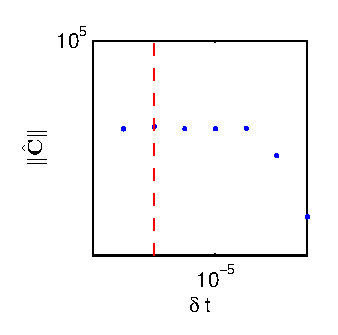
\epsfig{height=1.5in, file=C_dt_nonlinear_dt1_kernel1.eps}
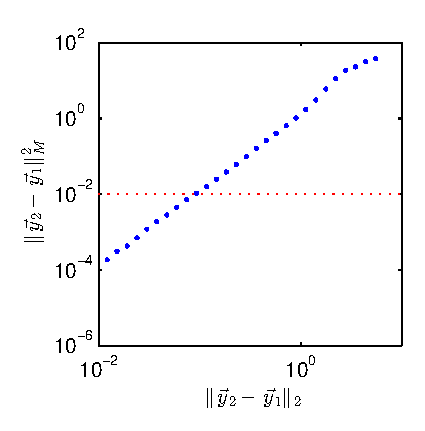
\epsfig{height=1.5in, file=dist_dy_nonlinear_dt1_kernel1.eps}
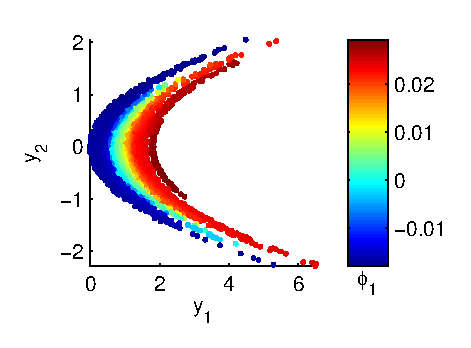
\epsfig{height=1.5in, file=data_nonlinear_NIV_dt1_kernel1.eps}

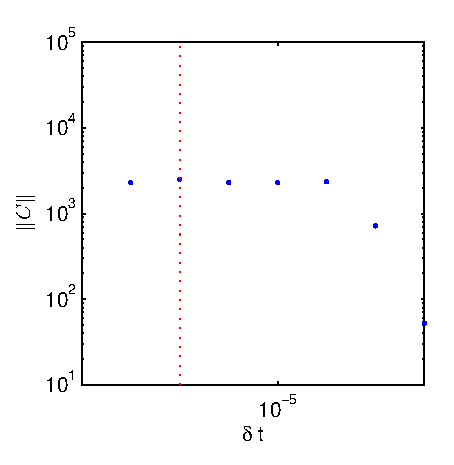
\epsfig{height=1.5in, file=C_dt_nonlinear_dt1_kernel2.eps}
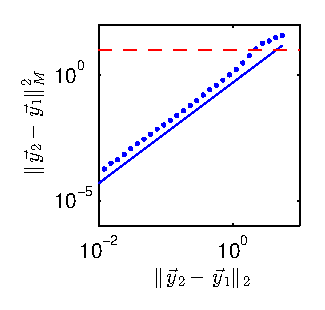
\epsfig{height=1.5in, file=dist_dy_nonlinear_dt1_kernel2.eps}
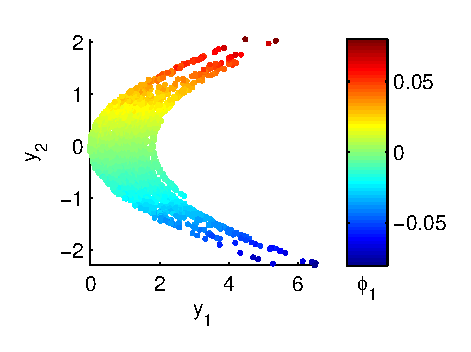
\epsfig{height=1.5in, file=data_nonlinear_NIV_dt1_kernel2.eps}

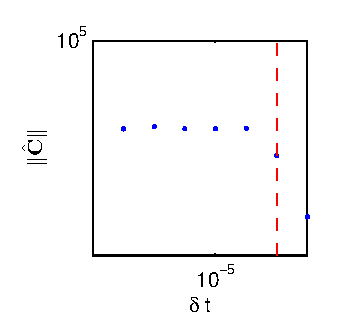
\epsfig{height=1.5in, file=C_dt_nonlinear_dt2_kernel1.eps}
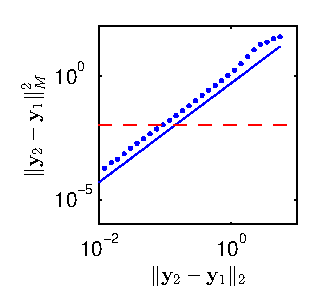
\epsfig{height=1.5in, file=dist_dy_nonlinear_dt2_kernel1.eps}
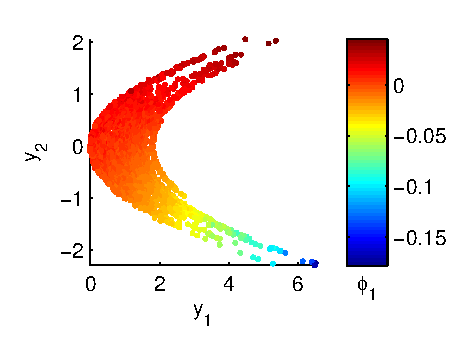
\epsfig{height=1.5in, file=data_nonlinear_NIV_dt2_kernel1.eps}

\caption{(a) Data from Figure~\ref{fig:initial_data_nonlinear}, colored by the first diffusion maps variable $\phi_1$ using the Mahalanobis distance with $\delta t = 10^{-7}$ and $\sigma_{kernel}^2 = 10^{-2}$. Note that the parametrization is one-to-one with the slow variable. (b) Data from Figure~\ref{fig:initial_data_nonlinear}, colored by $\phi_1$ using the Euclidean distance. We do not recover the slow variable, because the Euclidean distance is not informative as to the dynamics of the data. (c) Data from Figure~\ref{fig:initial_data_nonlinear}, colored by $\phi_1$ using the Mahalanobis distance with $\delta t = 10^{-7}$ and $\sigma_{kernel}^2 = 10^{1}$. We do not recover the slow variable because $\sigma_{kernel}$ is too large. (d) Data from Figure~\ref{fig:initial_data_nonlinear}, colored by $\phi_1$ using the Mahalanobis distance with $\delta t = 10^{-3}$ and $\sigma_{kernel}^2 = 10^{-2}$. We do not recover the slow variable because $\delta t$ is too large.  }
\label{fig:colored_data_nonlinear_cases}
\end{figure}


\section{Conclusion}

We showed that in certain cases (when we do {\em not} have a simulator where we can change $\delta t$), the data cannot be processed as-is (we cannot find the right kernel scale given a fixed $\delta t$ such that we can accurately recover the slow variable).

If the cloud of samples is too big then we can observe the cloud of clouds (and those clouds can be histograms, Fourier, scattering, etc.) as a way to get smaller clouds.


Richardson extrapolation could allow us to get an estimate of a second-order term in the covariance estimation, thereby locally approximating the function using a quadratic form, rather than a linear form,  which can lead to a better/improved/more accurate ``Mahalanobis'' metric.


\end{document}
